\documentclass[border=3pt]{standalone}
\usepackage{fontspec}
\setmainfont{Times New Roman}
\usepackage{pgfplots}
\pgfplotsset{compat=1.18}
\usetikzlibrary{arrows.meta,calc,positioning,shapes.geometric}
\definecolor{forest}{HTML}{346E57}
\definecolor{sage}{HTML}{E8EFEA}
\definecolor{clay}{HTML}{B77E60}
\definecolor{gray}{HTML}{718078}
\definecolor{rule}{HTML}{B7C3BA}
\definecolor{ink}{HTML}{000000}
\begin{document}
\hyphenpenalty=10000\exhyphenpenalty=10000
\fontsize{10}{12}\selectfont
\renewcommand{\small}{\fontsize{9}{11}\selectfont}
\renewcommand{\scriptsize}{\fontsize{8}{10}\selectfont}
\resizebox{16cm}{!}{%
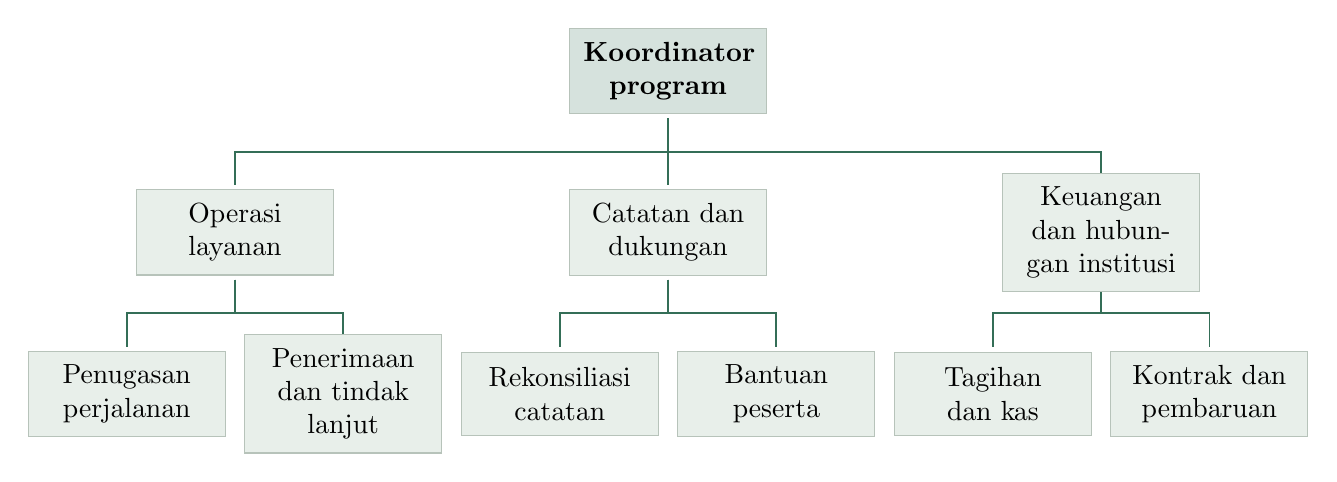
\begin{tikzpicture}[box/.style={draw=rule,fill=sage,text width=2.15cm,minimum height=1.05cm,align=center,inner sep=5pt},edge/.style={draw=forest,line width=.65pt}]
\draw[edge] (6.875,-0.6) -- (6.875,-1.025) -| (1.375,-1.4499999999999997);
\draw[edge] (6.875,-0.6) -- (6.875,-1.025) -| (6.875,-1.4499999999999997);
\draw[edge] (6.875,-0.6) -- (6.875,-1.025) -| (12.375,-1.4499999999999997);
\draw[edge] (1.375,-2.65) -- (1.375,-3.0749999999999997) -| (0.0,-3.4999999999999996);
\draw[edge] (1.375,-2.65) -- (1.375,-3.0749999999999997) -| (2.75,-3.4999999999999996);
\draw[edge] (6.875,-2.65) -- (6.875,-3.0749999999999997) -| (5.5,-3.4999999999999996);
\draw[edge] (6.875,-2.65) -- (6.875,-3.0749999999999997) -| (8.25,-3.4999999999999996);
\draw[edge] (12.375,-2.65) -- (12.375,-3.0749999999999997) -| (11.0,-3.4999999999999996);
\draw[edge] (12.375,-2.65) -- (12.375,-3.0749999999999997) -| (13.75,-3.4999999999999996);
\node[box] at (0.0,-4.1) {Penugasan perjalanan};
\node[box] at (2.75,-4.1) {Penerimaan dan tindak lanjut};
\node[box] at (1.375,-2.05) {Operasi layanan};
\node[box] at (5.5,-4.1) {Rekonsiliasi catatan};
\node[box] at (8.25,-4.1) {Bantuan peserta};
\node[box] at (6.875,-2.05) {Catatan dan dukungan};
\node[box] at (11.0,-4.1) {Tagihan dan kas};
\node[box] at (13.75,-4.1) {Kontrak dan pembaruan};
\node[box] at (12.375,-2.05) {Keuangan dan hubungan institusi};
\node[box,fill=forest!20,font=\bfseries] at (6.875,0.0) {Koordinator program};
\end{tikzpicture}
}

\end{document}
